\documentclass{article}
\usepackage[T1]{fontenc}
\usepackage[utf8]{inputenc}
\usepackage[margin=1in]{geometry}
\usepackage{fancyhdr} 
\usepackage{listings}
\usepackage{xcolor}

\definecolor{keywordcolor}{rgb}{0.4, 0.7, 1.0} % Light blue for keywords
\definecolor{ndkeywordcolor}{rgb}{0.8, 0.5, 0.0} % Orange for non-default keywords
\definecolor{stringcolor}{rgb}{0.8, 0.2, 0.2} % Red for strings
\definecolor{commentcolor}{rgb}{0.6, 0.6, 0.6} % Gray for comments
\definecolor{bracecolor}{rgb}{0.6, 0.6, 1.0} % Custom color for braces

\lstdefinelanguage{JavaScript}{
  keywords={break, case, catch, continue, debugger, default, delete, do, else, finally, for, function, if, in, instanceof, new, return, switch, this, throw, try, typeof, var, void, while, with},
  keywordstyle=\color{keywordcolor}\bfseries,
  ndkeywords={class, export, boolean, throw, implements, import, this},
  ndkeywordstyle=\color{ndkeywordcolor}\bfseries,
  identifierstyle=\color{black},
  sensitive=false,
  comment=[l]{//},
  morecomment=[s]{/*}{*/},
  commentstyle=\color{commentcolor}\itshape,
  stringstyle=\color{stringcolor}\ttfamily,
  morestring=[b]',
  morestring=[b]",
  literate={\{}{{\textcolor{bracecolor}{\{}}}1
           {\}}{{\textcolor{bracecolor}{\}}}}1
           {<}{{\textcolor{bracecolor}{<}}}1
           {>}{{\textcolor{bracecolor}{>}}}1,
}
\lstdefinelanguage{Python3}{
  keywords={False, async, class, finally, is, return, None, continue, for, lambda, try, True, def, from, nonlocal, while, and, del, global, not, with, as, elif, if, or, yield, assert, else, import, pass, break, except, in, raise},
  keywordstyle=\color{blue}\bfseries,
  ndkeywords={self},
  ndkeywordstyle=\color{darkgray}\bfseries,
  identifierstyle=\color{black},
  sensitive=true,
  comment=[l]{\#},
  morecomment=[s]{"""}{"""},
  commentstyle=\color{purple}\ttfamily,
  stringstyle=\color{red}\ttfamily,
  morestring=[b]',
  morestring=[b]",
  emph={print, len, range, int, str, float, list, dict, set, tuple},
  emphstyle={\color{teal}}
}
\usepackage[ruled,vlined]{algorithm2e}
\usepackage{amsthm}
\usepackage{amsfonts}
\usepackage{amssymb}
\usepackage{graphicx}
\usepackage[dvipsnames]{xcolor}
\usepackage{xy}
% \usepackage{url} % Commented out because hyperref provides similar functionality
\usepackage{parskip}
\usepackage{comment}
\usepackage{setspace}
\usepackage{enumerate}
\usepackage{multirow}
\usepackage{hyperref}
\usepackage{caption}
\usepackage{subcaption}
\usepackage{booktabs}
\usepackage{wrapfig}
\usepackage{times}

\captionsetup[figure]{font={small,it}}

\usepackage[backend=biber,style=numeric,sortcites,maxbibnames=99]{biblatex}
\addbibresource{references.bib}

\newcommand{\HRule}{\rule{\linewidth}{0.5mm}}
\newcommand{\Hrule}{\rule{\linewidth}{0.3mm}}
\newcommand{\classnum}{CS-GY 6313 B}

\makeatletter% since there's an at-sign (@) in the command name
\renewcommand{\@maketitle}{%
  \parindent=0pt% don't indent paragraphs in the title block
  \centering
  {\Large \bfseries\textsc{\@title}}
  \HRule\par%
  \textit{\@author \hfill \classnum}
  \par
}
\makeatother% resets the meaning of the at-sign (@)

\title{Assignment 4: Data Viz for Advocacy} 
\author{Ivan Aristy — iae225}
% \classnum

\begin{document}
  \maketitle % prints the title block
  \thispagestyle{empty}
  % \vspace{-15pt}

\section{Interactive Visualization}

\subsection{Question}
\label{subsec:subsec1}

\textbf{How are men's mental states in the US?}

The question is a bit general, but I want to communicate to a general audience
that is not aware of the high levels of mental health issues that men face in the US.

\subsection{Data}
\label{subsec:subsec2}

\subsubsection{Data Source}
\label{subsubsec:Data Source}

There are a few data sources to get information from.

The CDC holds lots of information, but particularly I looked into:

\begin{enumerate}
  \item Behavioral Risk Factor Surveillance System (BRFSS) Survey
  \item Household Pulse Survey
  \item National Health and Nutrition Examination Survey (NHANES)
  \item National Health Interview Survey (NHIS)
\end{enumerate}

However, much to my dismay, lot's of the Data I was looking for 
was not available. I was able to retrieve information for suicide rates,
but the data regarding mental health for men was quite limited.

I ended up using \url{https://www.cdc.gov/suicide/facts/data.html#cdc_data_surveillance_section_4-suicide-rates}
for suicide rate information, and \url{https://www.apa.org/monitor/2015/12/numbers}
for general information and stats regarding suicide rates.

\subsubsection{Serving Information} 
\label{subsubsec:Serving Backend Server}

For serving information, we use D3's csv function:

\begin{lstlisting}[language=JavaScript]
  import * as d3 from "d3";
  import { Dataset } from "@/types/types";
  import theme from "@/types/themes";
  
  export async function loadRatesData(): Promise<Dataset[]> {
    const data = await d3.csv("/rates.csv", d3.autoType); 
    console.log(data); 
  
    return [
      {
        label: "Total Population",
        data: data.map((d: any) => ({ x: d["Year"],
         y: d["Total Population"] })), 
        color: "#d4c2d4", 
      },
      {
        label: "Male",
        data: data.map((d: any) => ({ x: d["Year"], y: d["Male"] })),
        color: "#cbd4c2", 
      },
      {
        label: "Female",
        data: data.map((d: any) => ({ x: d["Year"], y: d["Female"] })), 
        color: "#c2c2d4", 
      },
    ];
  }  
\end{lstlisting}

and pass the data to the chart component through a wrapper.

\subsection{Visualization}
\label{subsec:Visualization}

\subsubsection{Frontend Setup}
\label{subsubsec:Frontend}

The frontend is a simple NextJS application that uses the 
\texttt{D3} library to create the chart, and react hooks to update 
and keep track of state.

My main secondary goal for this visualization was to make the 
design look sleek and simple. 

As opposed to my previous visualization, I wanted to make a website that
was more visually appealing and easier to understand, as well as having 
goodies like smooth transitions and a responsive design.

For smooth transitions I used the Lenis library, which allowed for smooth 
scrolling. This greatly improved the feel of the website, and allowed me 
to dynamically render the chart when the user scrolls to the chart section.

\begin{lstlisting}[language=JavaScript]
const [isVisible, setIsVisible] = useState(false);
    const ref = useRef<HTMLDivElement>(null);
  
    // Lenis hook to listen for scroll events
    useLenis(() => {
      if (ref.current && !isVisible) {
        const { top, bottom } = ref.current.getBoundingClientRect();
        const windowHeight = window.innerHeight;
  
        if (top + 300 < windowHeight && bottom > 0) {
          setIsVisible(true);
        }
      }
    });
\end{lstlisting}

\subsubsection{Components}
\label{subsubsec:Components}

To allow for interactivity, we create a few drop down labels that allow the user
to select the data that they want to plot. For example, here is the code
for the "Champion" Label:

\begin{lstlisting}[language=JavaScript]
  <label>
    Champion:
    <select
      value={selectedChampion}
      onChange={(e) => setSelectedChampion(e.target.value)}
    >
      {champions.map((champ) => (
        <option key={champ} value={champ}>
          {champ}
        </option>
      ))}
    </select>
  </label>
\end{lstlisting}

This also allows you to type out the champion name 
instead of going through every single champion in the dropdown.

Additionally, I implemented another QoL feature that deals with situations
where the user selects a patch range that is not valid. 
For example, if the user sets start patch to 14.20 and end patch is at 14.10,
the code will automatically adjust the end patch to 14.20.

\subsubsection{Visualization Logic}
\label{subsubsec:Visualization Logic}

I revisited D3 to create a custom chart, building upon my previous 
experience with the library. 

Working directly with D3 again proved to be more challenging 
but also rewarding, as it deepened my understanding of chart components 
and their implementation.

I gained a more explicit appreciation for the building blocks of a chart:

\begin{itemize}
  \item Margins: Carefully planned margins to ensure sufficient space for elements like axes, labels, and legends.
  \item Scales: Mapped dynamically to the data, ensuring that the chart is responsive to changes in data.
  \item Line: This time, I used 3 lines to represent the data, each with a different color.
  \item Tooltip:
  \item Circles: Since we were using 3 lines and transitions, the circles 
  \item Dynamics: I progresively drew the lines, and added a transition to make the chart more visually appealing. 
  I also believe that this draws attention to the chart, as the user is more likely to notice the chart if it is moving.
  Plus it highlights how rates increase over time.
  \item Axes: Created axes, gridlines, and basic labels for 
  intuitive and fast understanding by the user.
\end{itemize}

\subsection{Improvements}
\label{subsec:Improvements}

\subsubsection{Champion Image}
\label{subsubsec:Champion Image}

A major piece of feedback was to include the champion image in the visualization.
This would allow the user to quickly identify the champion they are looking at,
not having to rely on the champion name alone, which could be pretty small on 
some devices.

This was actually added.

\subsubsection{Small Patch Ranges}
\label{subsubsec:Small Patch Ranges}

We have a degenerate case where the user selects a patch range that is so small
that visualizing it in a line chart is not very useful.

See \autoref{fig:fig2} and \autoref{fig:fig3} for an example of this.

\begin{figure}[ht] 
  \centering
  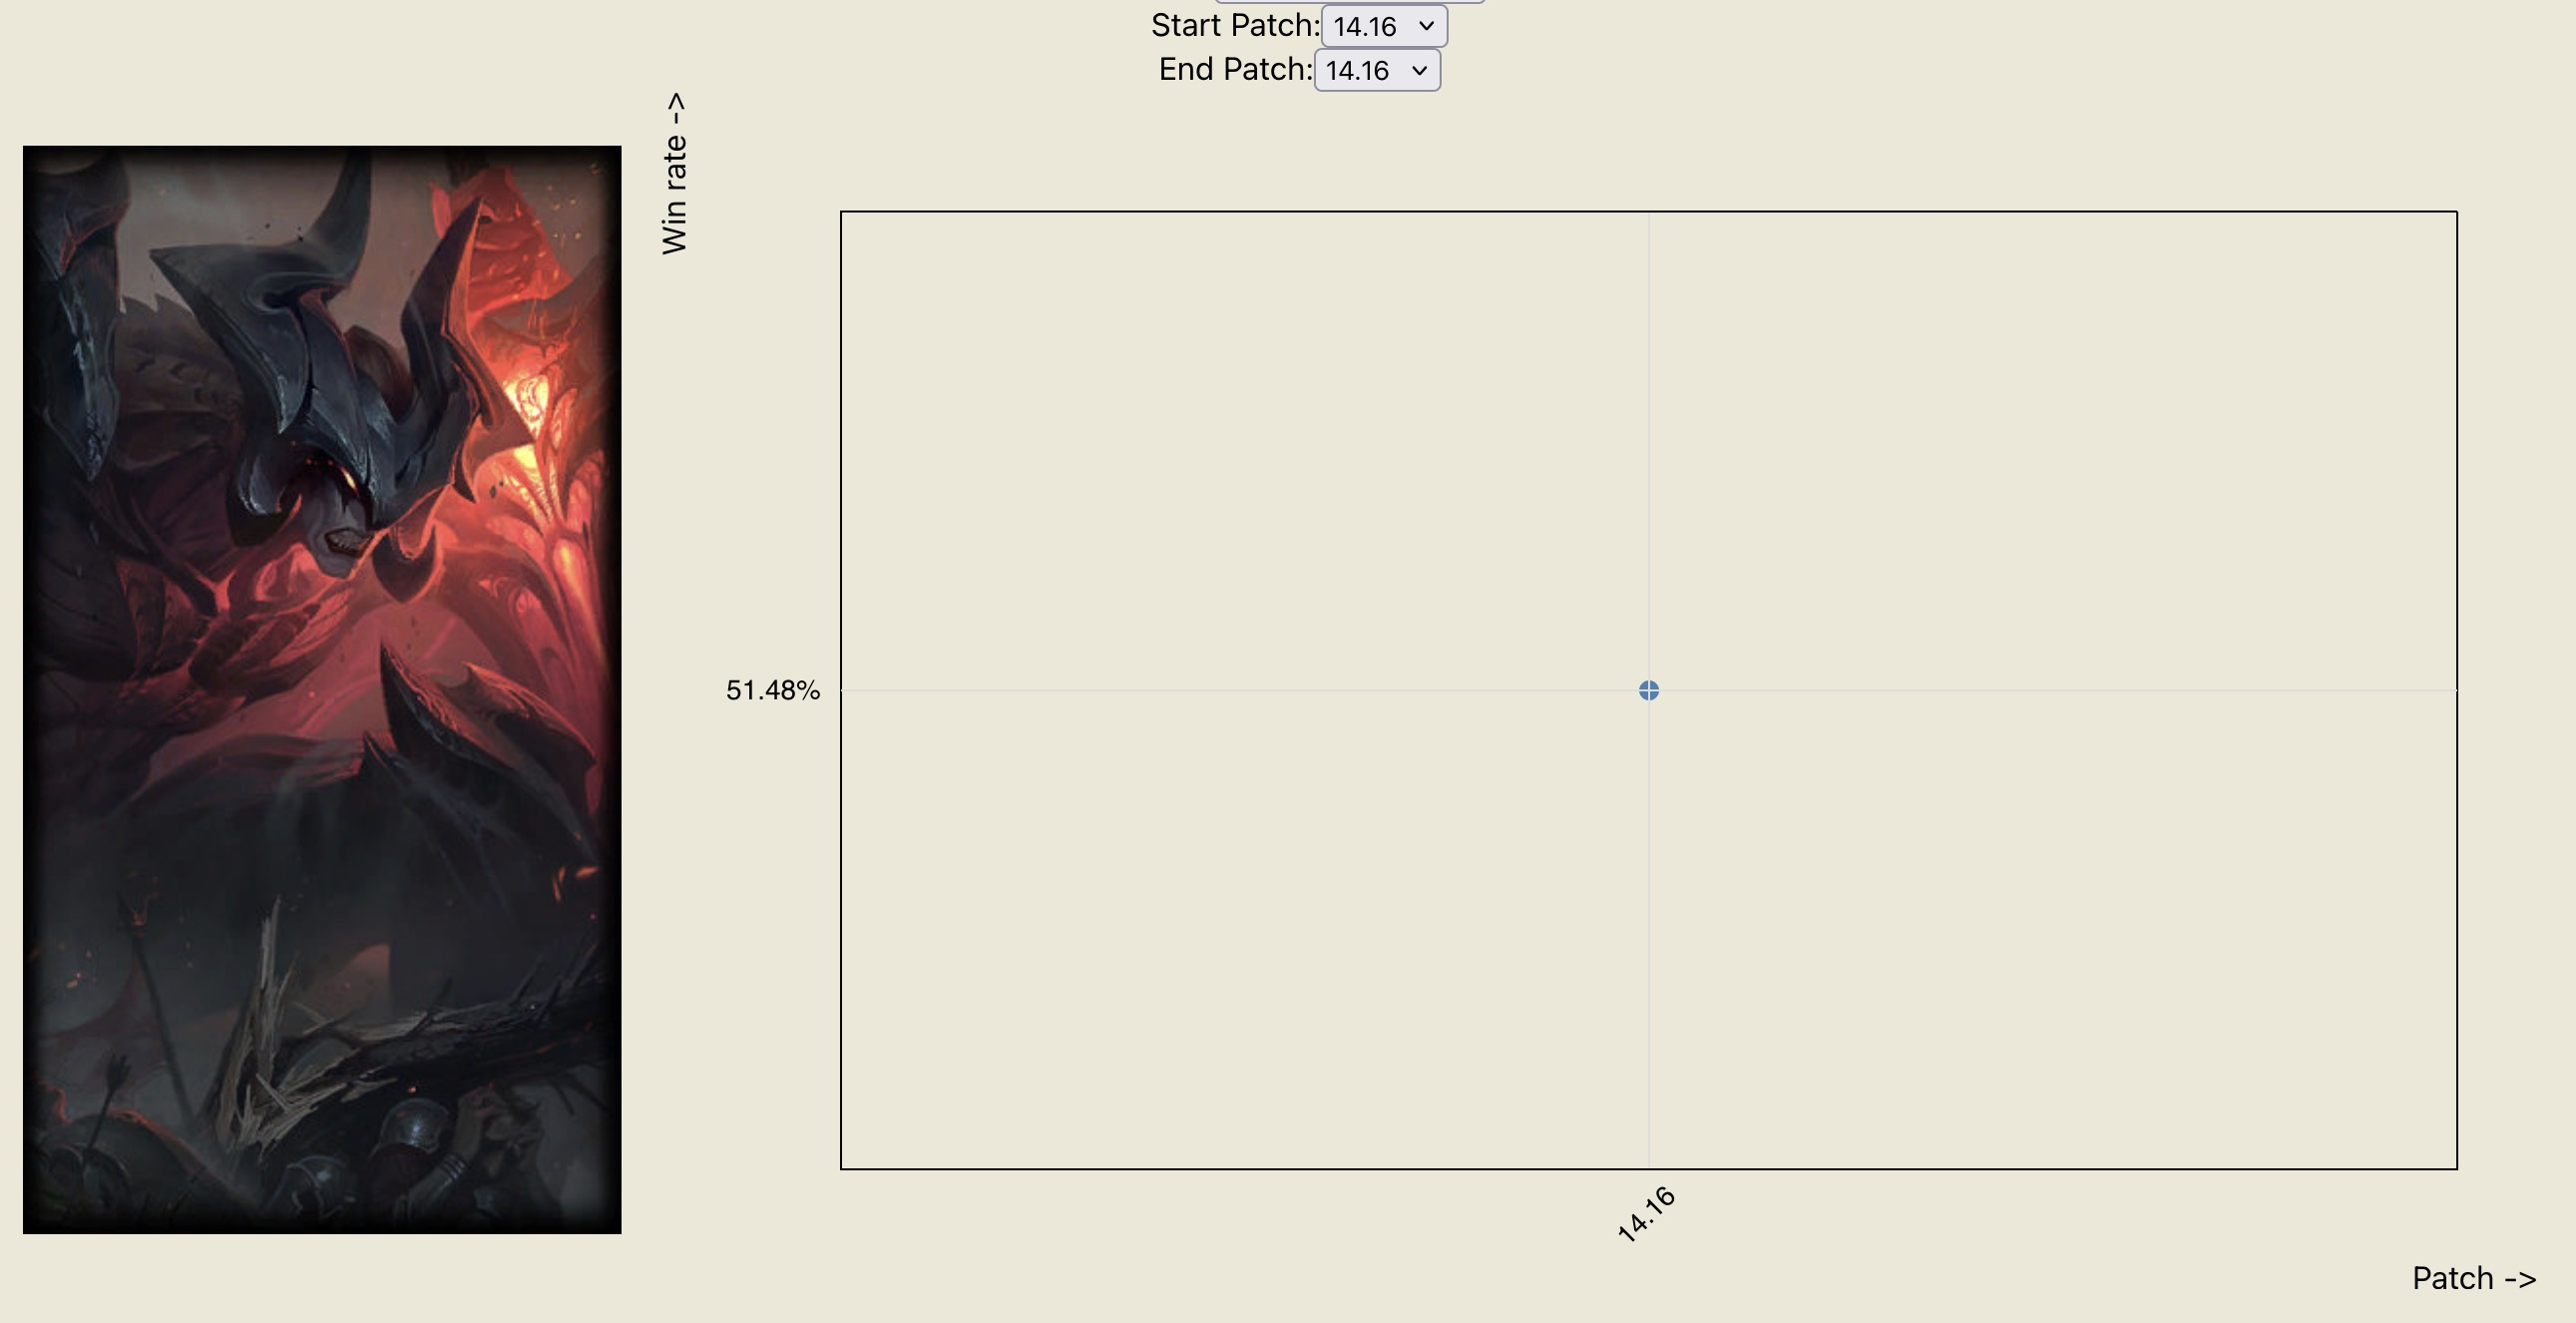
\includegraphics[width=0.75\textwidth]{figs/one.jpg}
  \caption{
      Solo patch range.
  }
  \label{fig:fig2}
\end{figure}

\begin{figure}[ht] 
  \centering
  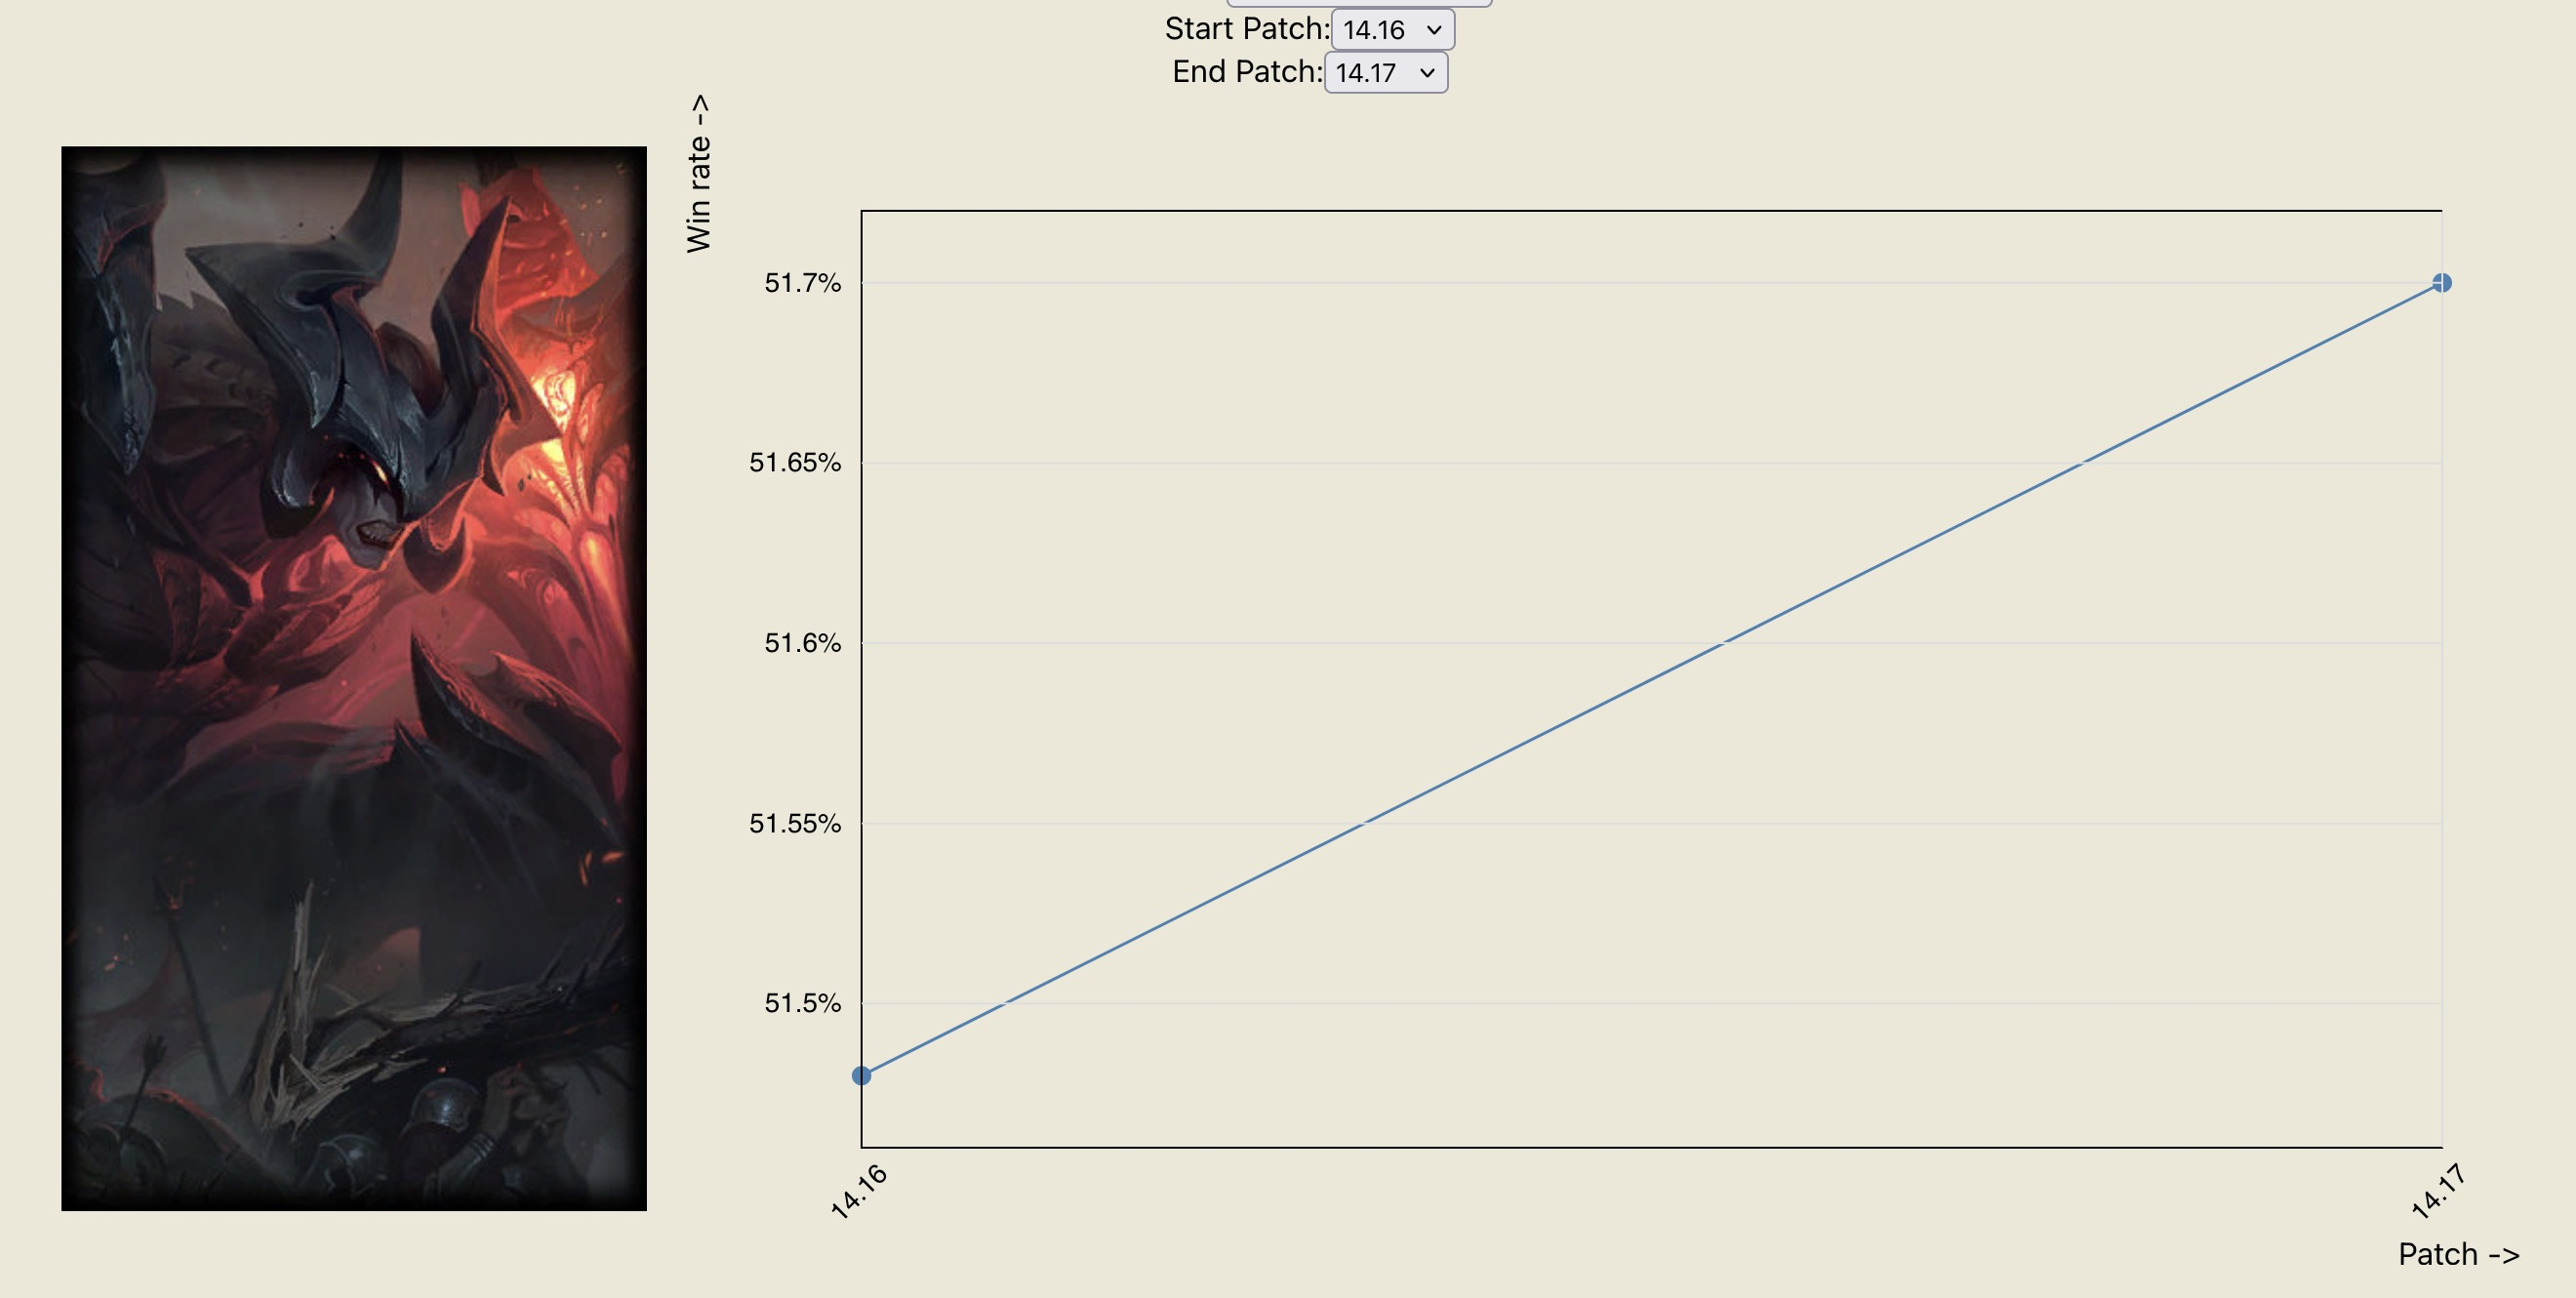
\includegraphics[width=0.75\textwidth]{figs/two.jpg}
  \caption{
      Size 2 patch range.
  }
  \label{fig:fig3}
\end{figure}

I did not create a fix for this specific situation, since the Visualization is 
for users to see how their champion has been impacted over time.

\subsubsection{Lane Specific Data}
\label{subsubsec:Lane Specific Data}

Another piece of feedback was to include lane specific data.

Why? Well, a botlane champion will have a different winrate if they are played toplane. 
In layman's terms, the best pizza is not a very good burger. 
Also, some champions are played in multiple lanes, so it would be interesting to see
how their winrate changes depending on the lane.

I deemed this to be beyond the scope of the assignment, but it is a good idea.

\subsection{Conclusion: Do we answer the question?}
\label{subsec:Conclusion}

I believe for both:


\begin{refcontext}[sorting=nyt]
\printbibliography
\end{refcontext}

\end{document}

